\documentclass[onecolumn, draftclsnofoot,10pt, compsoc]{IEEEtran}
\usepackage{graphicx}
\usepackage{url}
\usepackage{setspace}

\usepackage{geometry}
\geometry{textheight=9.5in, textwidth=7in}

\def \CapstoneTeamName{		100k Challenge CS}
\def \CapstoneTeamNumber{		42}
\def \GroupMemberOne{			Glenn Upthagrove}
\def \GroupMemberTwo{		 	Sam Hudson}
\def \GroupMemberThree{			Michael Elliott}
\def \CapstoneProjectName{		100K Spaceport America Demonstration Rocket Project}
\def \CapstoneSponsorCompany{	School of Mechanical Engineering, Oregon State University}
\def \CapstoneSponsorPerson{		Nancy Squires}

% 2. Uncomment the appropriate line below so that the document type works
\def \DocType{  %Problem Statement
				Requirements Document
				%Technology Review
				%Design Document
				%Progress Report
				}
			
\newcommand{\NameSigPair}[1]{\par
\makebox[2.75in][r]{#1} \hfil 	\makebox[3.25in]{\makebox[2.25in]{\hrulefill} \hfill		\makebox[.75in]{\hrulefill}}
\par\vspace{-12pt} \textit{\tiny\noindent
\makebox[2.75in]{} \hfil		\makebox[3.25in]{\makebox[2.25in][r]{Signature} \hfill	\makebox[.75in][r]{Date}}}}
% 3. If the document is not to be signed, uncomment the RENEWcommand below
%\renewcommand{\NameSigPair}[1]{#1}

%%%%%%%%%%%%%%%%%%%%%%%%%%%%%%%%%%%%%%%
\begin{document}
\begin{titlepage}
    \pagenumbering{gobble}
    \begin{singlespace}
    	
\includegraphics[height=4cm]{coe_v_spot1}
        \hfill 
        % 4. If you have a logo, use this includegraphics command to put it on the coversheet.
        %\includegraphics[height=4cm]{CompanyLogo}   
        \par\vspace{.2in}
        \centering
        \scshape{
            \huge CS Capstone \DocType \par
            {\large\today}\par
            \vspace{.5in}
            \textbf{\Huge\CapstoneProjectName}\par
            \vfill
            {\large Prepared for}\par
            \Huge \CapstoneSponsorCompany\par
            \vspace{5pt}
            {\Large\NameSigPair{\CapstoneSponsorPerson}\par}
            {\large Prepared by }\par
            Group\CapstoneTeamNumber\par
            % 5. comment out the line below this one if you do not wish to name your team
            \CapstoneTeamName\par 
            \vspace{5pt}
            {\Large
                \NameSigPair{\GroupMemberOne}\par
                \NameSigPair{\GroupMemberTwo}\par
                \NameSigPair{\GroupMemberThree}\par
            }
            \vspace{20pt}
        }
        \begin{abstract}
        % 6. Fill in your abstract    
        The Transmission protocol and Kalman filter we shall maximize data integrity. The
        Ground Station shall collect the data in near real time, and display this data to the screen at a
        constant refresh rate. The visualization will be human readable and display the best known
        approximation of the position of the rocket. The following details the features and
        expectations of the software we shall be developing.\par
        \end{abstract}     
    \end{singlespace}
\end{titlepage}
\newpage
\pagenumbering{arabic}
\tableofcontents
% 7. uncomment this (if applicable). Consider adding a page break.
%\listoffigures
%\listoftables
\clearpage

\section{Introduction}
\subsection{Purpose}
This document shall serve going forth as a description of the requirements and
expectations of the software created by the computer science sub team for the 100k rocketry
challenge.
\subsection{Scope}
The software created by this sub-team shall, in conjunction with electrical sub-
team, create a transmission protocol and Kalman filter to transmit and receive the data as
accurately as possible. The data shall be stored on the ground station. There shall also be a
visualization that can present this data to the user. This implies:
 \begin{enumerate}
    \item The rocket can be tracked and recovers.
    \item The highest altitude can be recorded.
    \item The user will be able to view the data at a rate that is readable.
 \end{enumerate}
\subsection{Definitions and Acronyms}
Blackout: A long period where no data is recovered. \par
Corruption: When data in transmission changes value due to interference. \par
Data: Measurements of importance. \par
GS: Ground Station, a computer on the ground used during the flight. \par
GUI: Graphical User Interface. A visual interface with the software. \par
JSON: JavaScript Object Notation. A way of annotating data. \par
Kalman Filter: A system which uses both data and an ideal model to make a best estimate. \par
KATE: A software package for making announcements at certain altitudes. \par
Noise: Improper readings from sensors due to its constraints. \par
Packet: a complete set of data that is transmitted. \par
Packet Loss: When a packet does not reach the destination. \par
Protocol: The system for packaging and transmitting the telemetry data. \par
Serial: Data transferred sequentially over a single data line. \par
Telemetry: The data used for tracking the data. \par
\subsection{Overview}
The remainder of this document describes in more detail the aspects and
requirements of the software. This shall involve the interaction between our software and the
other aspects of the project. The following section, \textit{Overall Description}, shall give a broad
description of what our software shall do and the factors we must work with. The last section,
\textit{Specific Requirements}, shall put forth in detail the exact expectations of the software we shall
deliver.
\section{Overall Description}
\subsection{Product Perspective}
The transmission protocol shall transmit the data from the rocket to
the GS as accurately as possible. There shall also be a Kalman filter that will help to keep the
data accurate beyond the capabilities of the protocol and the noise associated with the
sensors. The GS will receive data via a wireless interface with the rocket. The data will be
transmitted in a serial fashion. The ground station will not be connected to the Internet, and
shall be in communication only with the rocket. The data the GS receives from the rocket shall
be stored, and used to update the visualization shown to the user.
\subsection{Product Functions: The software shall provide several features}
 \begin{enumerate}
    \item The data shall be collected and stored for later use.
    \item The data shall be displayed to the user in near real time.
    \item The data can be used later to create a 3D trace of the flight path.
 \end{enumerate}
\subsection{User Characteristics}
The GS shall be used only by people associated with this
challenge, and thus have some level of technical knowledge. The visualization and 3D trace
should, however, also easily readable by anyone.
\subsection{Constraints}
 \begin{enumerate}
    \item Due to the altitude the rocket shall theoretically reach, there is a significant chance that
packet loss and blackout could occur.
    \item Due to the body of the rocket being in large part carbon fiber, there is a chance this could
also cause packet loss.
    \item The rocket has limited processing power.
    \item The ground station will also not be very powerful.
 \end{enumerate}
\subsection{Assumptions and Dependencies}
We assume the rocket shall be using a Telemega chip. We also assume that the GS will be
based off of a Raspberry Pi, running a distortion of Linux.
\subsection{Apportioning of Requirements}
There is a gantt chart in figure 1. This outlines the time line for our software from now until the
test launch. Our software must be at a stable state by the test launch so it can be used to full
effect at that time.
\section{Specific Requirements}
\subsection{Protocol Requirements} The protocol will be able, as long as there is a connection, to
transmit a full set of telemetry data at least once per second. The packets shall also be
packaged in a JSON or similar format.

\subsection{GS Requirements}
The GS shall be able to display a visualization and update the
visualization once per second.
\subsection{Visualization Requirements}
The visualization will be human readable. This will be
defined by at least 6 out of 10 people asked to review the visualization agreeing. These
people will not be EECS majors, nor in similar fields. There will be an update once per
second. This will make the visualization near real time.
\subsection{3D Trace Requirements}
The trace shall be able to read the recorded data after the flight
and display the flight path in 3D space.
\subsection{Near Real Time 3D Trace (Stretch Goal)}
The trace can display the flight path in near
real time as the data is received on the GS.
\subsection{KATE Integration (Stretch Goal)}
We shall integrate KATE into our GS.

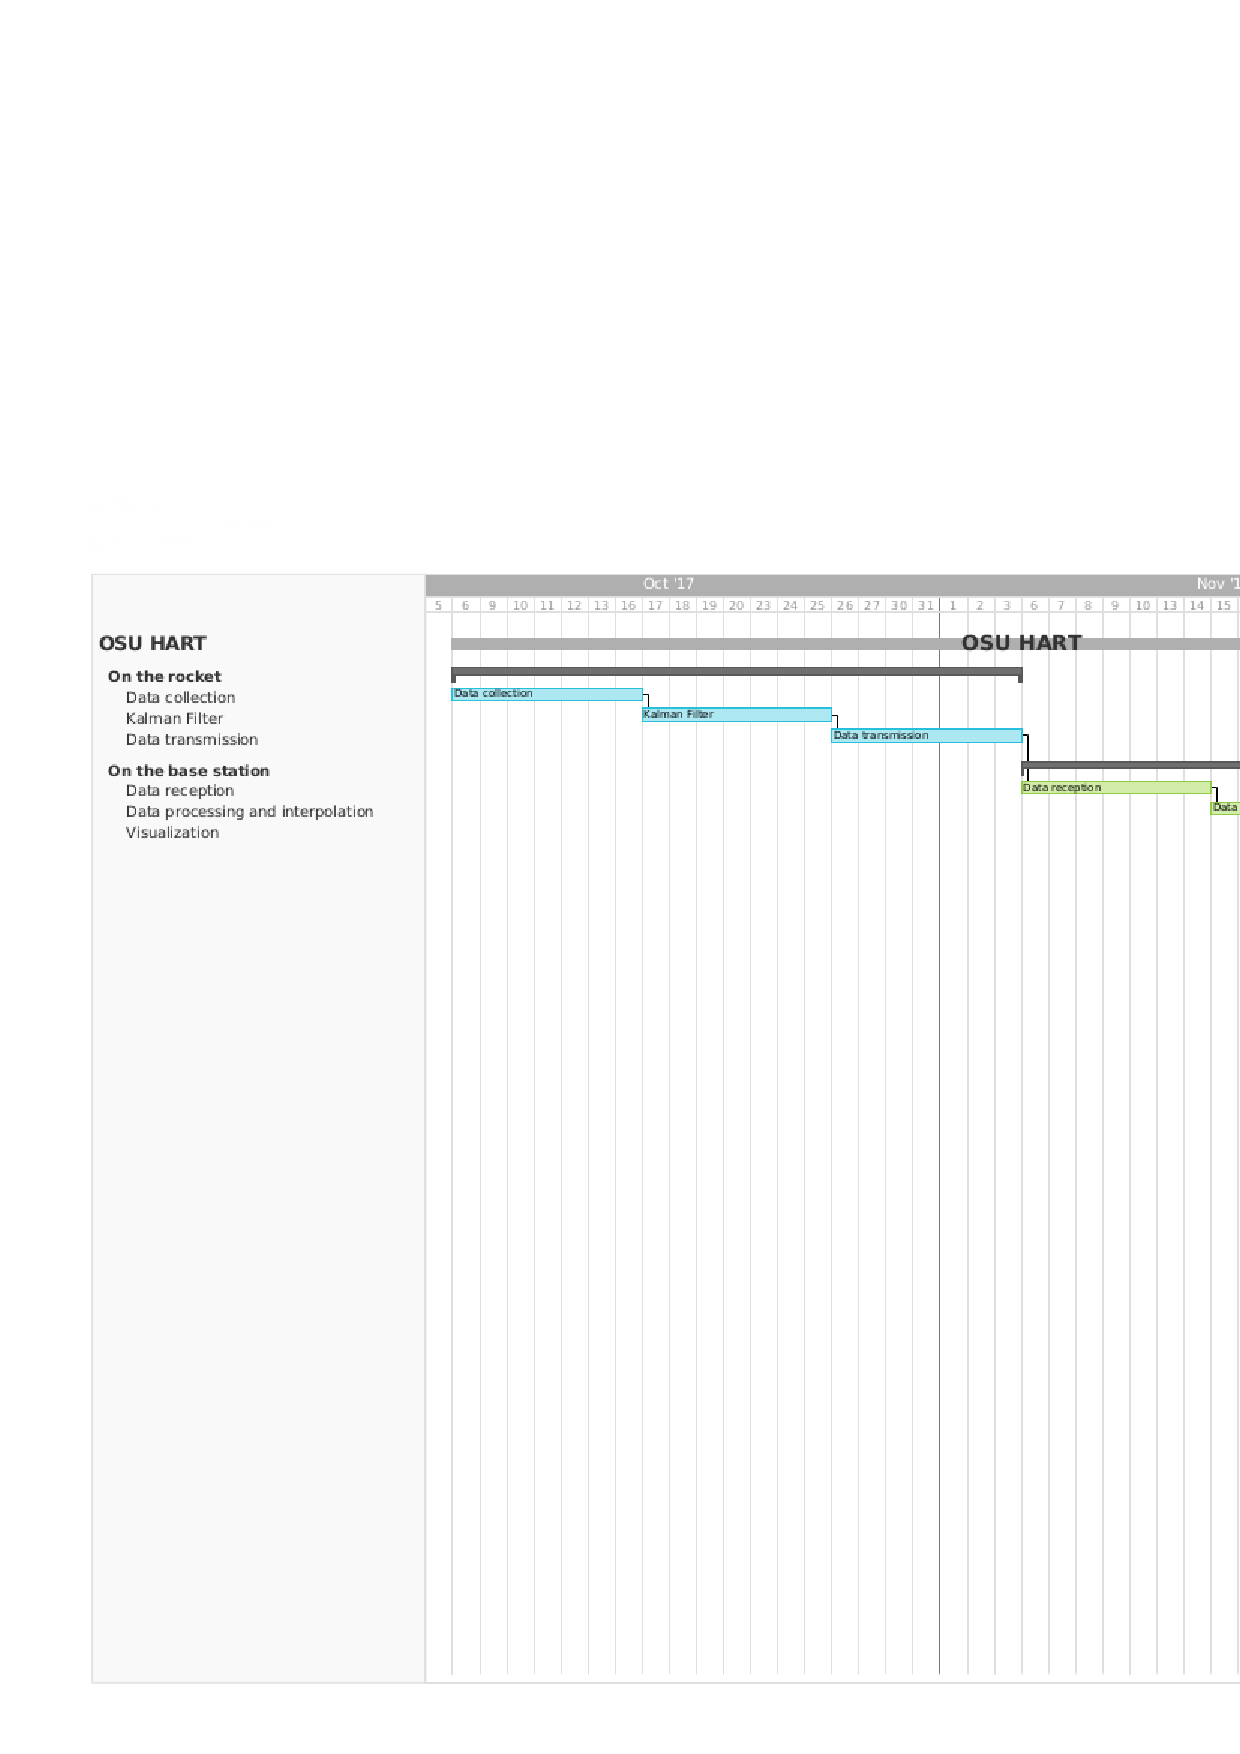
\includegraphics[width=\textwidth,height=\textheight]{gantt}

\end{document}
